\chapter{FPGA Design \& Implementation} 
% architecutr &design & impementation
\label{Chapter-FPGA-Implementation}

\section{Tools Used}
\subsection{Vitis Unified Software Platform}
The Vitis unified software platform\cite{Vitis_unified_software_platform} is a collection of tools, libraries and environments designed to ease the development of accelerated applications tailored for AMD Xilinx FPGA and Versal® ACAP hardware platforms. It includes graphical and command-line compilers, analyzers, and debuggers to build applications, analyze performance bottlenecks, and debug accelerated algorithms, developed in C, C++, or OpenCL APIs. Furthermore, it offers numerous advantages such as effortless application portability, complete simulation of hardware systems, and an open source runtime that handles host-device communication.
\begin{figure}[H]
    \centering
        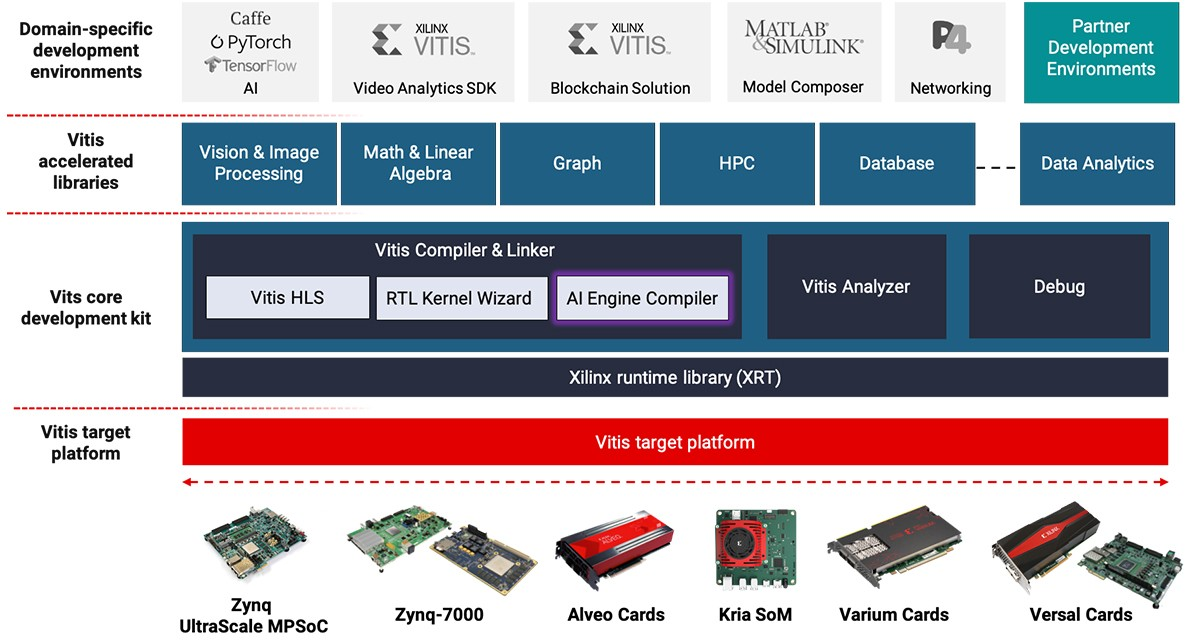
\includegraphics[width=1\textwidth]{Images/Platform/vitis.jpg}
        \decoRule
        \caption[Vitis]{Vitis overview: \href{https://www.xilinx.com/products/design-tools/vitis/vitis-platform.html\#overview}{URL}.}
        \label{fig:Vitis_overview}
\end{figure}

Vitis supports hardware acceleration kernels controlled by PS or x86 kernels. The Vitis application acceleration development flow provides a framework for developing and delivering FPGA-accelerated applications using standard programming languages for both software and hardware components. The kernels can be developed through traditional RTL, C/C++ with Vitis HLS, the Vitis model composer and the AI Engine compiler.
\begin{figure}[H]
    \centering
        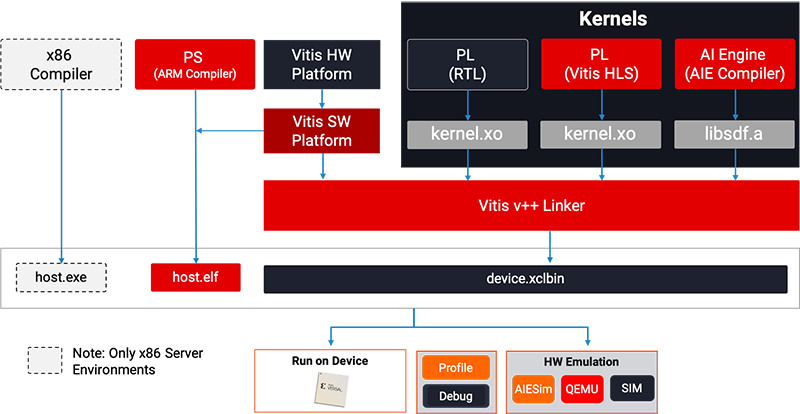
\includegraphics[width=1\textwidth]{Images/Platform/vitis_kernel.png}
        \decoRule
        \caption[Vitis]{Vitis kernel architecture: \href{https://www.xilinx.com/products/design-tools/vitis/vitis-platform.html\#development}{URL}.}
        \label{fig:Vitis_kernel_overview}
\end{figure}

\subsection{Xilinx Runtime library (XRT)}
The Xilinx Runtime library\cite{Xilinx_Runtime_Library} (XRT) facilitates communication between the application code (running on an embedded Arm or x86 host) and the accelerators deployed on the reconfigurable portion of PCIe interface-based AMD Xilinx accelerator cards, MPSoC-based embedded platforms, or ACAPs. It is flexible with modifiable libraries and drivers, enabling different levels of abstractions, from high-level Python bindings to low-level C++ APIs. Its APIs are common across all platforms and require no hardware expertise, eliminating the need to implement hardware communication layers from scratch.
\begin{figure}[H]
    \centering
        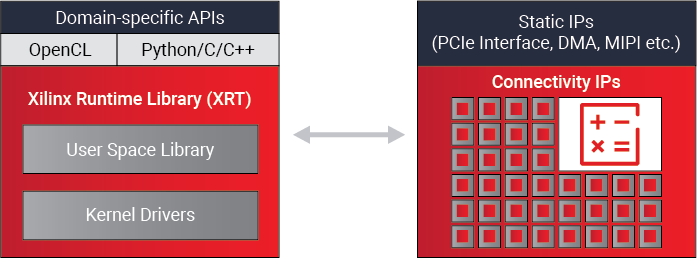
\includegraphics[width=1\textwidth]{Images/Platform/xrt.png}
        \decoRule
        \caption[Xilinx Runtime Library]{Xilinx Runtime Library overview: \href{https://www.xilinx.com/products/design-tools/vitis/xrt.html}{URL}.}
        \label{fig:XRT_overview}
\end{figure}

\subsection{Vitis High Level Synthesis (HLS)}

\section{FPGA Platforms}
